\documentclass{standalone}
\usepackage{tikz}
\usetikzlibrary{patterns, positioning}


\begin{document}
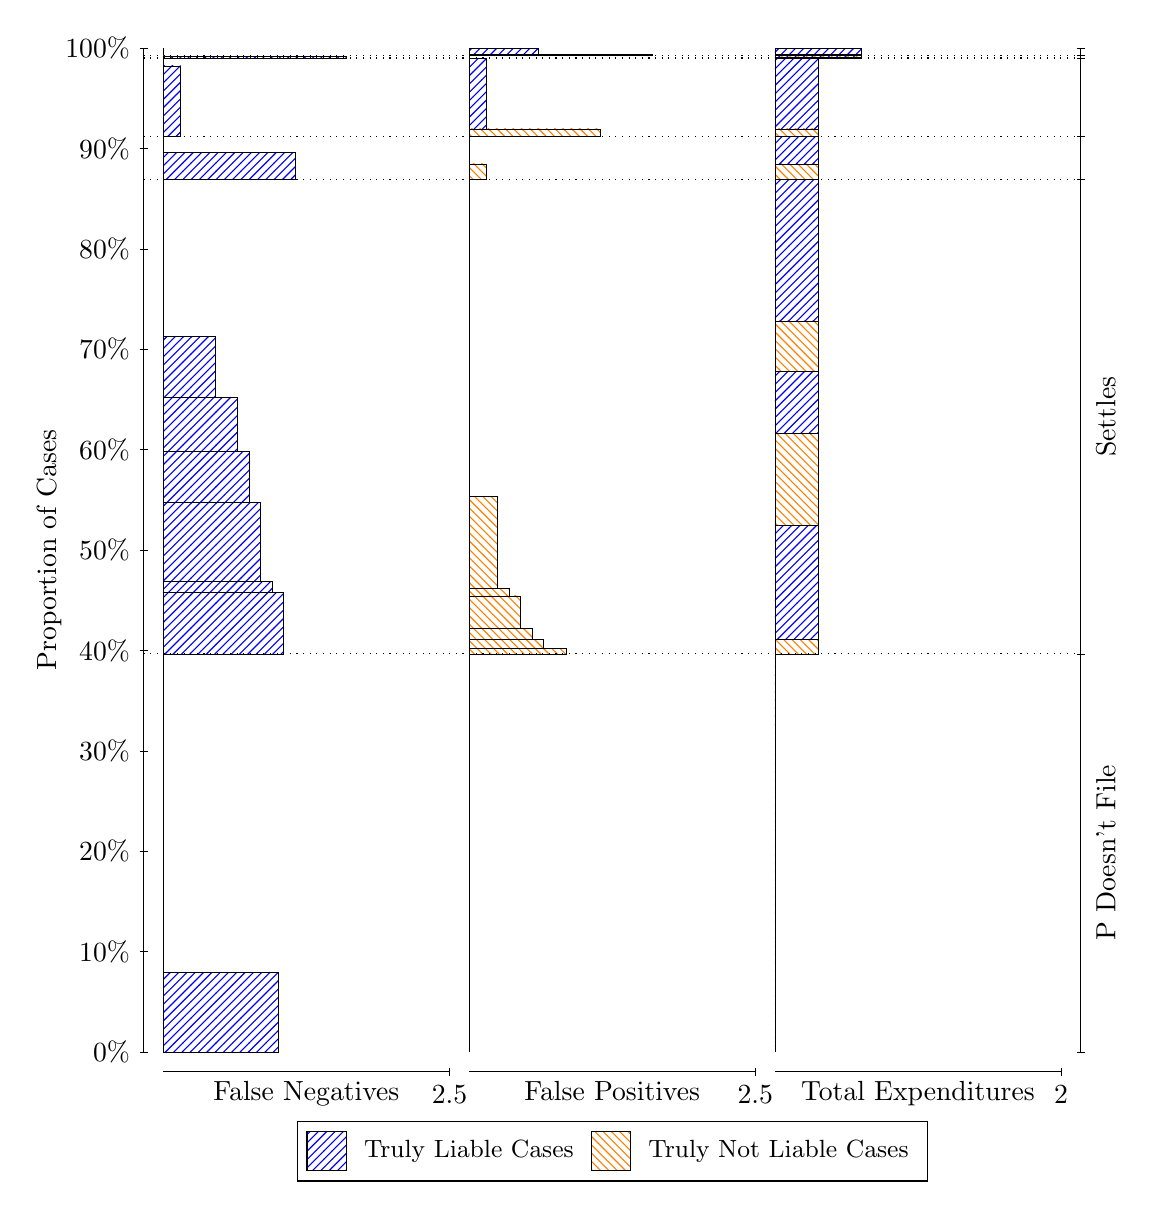
\begin{tikzpicture}
\draw[black, very thin] (1.5,1.75) -- (1.5,14.5);
\node[rotate=90, text=black, anchor=center] at (0.3, 8.125) {Proportion of Cases};
\draw[black, very thin] (1.45,1.75) -- (1.55,1.75);
\node[text=black, anchor=east] at (1.45, 1.75) {0\%};
\draw[black, very thin] (1.45,3.025) -- (1.55,3.025);
\node[text=black, anchor=east] at (1.45, 3.025) {10\%};
\draw[black, very thin] (1.45,4.3) -- (1.55,4.3);
\node[text=black, anchor=east] at (1.45, 4.3) {20\%};
\draw[black, very thin] (1.45,5.575) -- (1.55,5.575);
\node[text=black, anchor=east] at (1.45, 5.575) {30\%};
\draw[black, very thin] (1.45,6.85) -- (1.55,6.85);
\node[text=black, anchor=east] at (1.45, 6.85) {40\%};
\draw[black, very thin] (1.45,8.125) -- (1.55,8.125);
\node[text=black, anchor=east] at (1.45, 8.125) {50\%};
\draw[black, very thin] (1.45,9.4) -- (1.55,9.4);
\node[text=black, anchor=east] at (1.45, 9.4) {60\%};
\draw[black, very thin] (1.45,10.675) -- (1.55,10.675);
\node[text=black, anchor=east] at (1.45, 10.675) {70\%};
\draw[black, very thin] (1.45,11.95) -- (1.55,11.95);
\node[text=black, anchor=east] at (1.45, 11.95) {80\%};
\draw[black, very thin] (1.45,13.225) -- (1.55,13.225);
\node[text=black, anchor=east] at (1.45, 13.225) {90\%};
\draw[black, very thin] (1.45,14.5) -- (1.55,14.5);
\node[text=black, anchor=east] at (1.45, 14.5) {100\%};

\draw[black, very thin] (13.4,1.75) -- (13.4,14.5);
\draw[black, very thin] (13.35,1.75) -- (13.45,1.75);
\node[anchor=west] at (13.35, 1.75) {};
\draw[black, very thin] (13.35,6.8066) -- (13.45,6.8066);
\node[anchor=west] at (13.35, 6.8066) {};
\draw[black, very thin] (13.35,12.828) -- (13.45,12.828);
\node[anchor=west] at (13.35, 12.828) {};
\draw[black, very thin] (13.35,13.373) -- (13.45,13.373);
\node[anchor=west] at (13.35, 13.373) {};
\draw[black, very thin] (13.35,14.373) -- (13.45,14.373);
\node[anchor=west] at (13.35, 14.373) {};
\draw[black, very thin] (13.35,14.405) -- (13.45,14.405);
\node[anchor=west] at (13.35, 14.405) {};
\draw[black, very thin] (13.35,14.5) -- (13.45,14.5);
\node[anchor=west] at (13.35, 14.5) {};

\draw[black, very thin, pattern color=blue, pattern=north east lines] (1.75,1.75) rectangle (3.2033,2.7584);
\draw[black, very thin, pattern color=orange, pattern=north west lines] (1.75,2.7584) rectangle (1.75,6.8067);
\draw[black, very thin, pattern color=blue, pattern=north east lines] (1.75,6.8067) rectangle (3.276,7.5889);
\draw[black, very thin, pattern color=blue, pattern=north east lines] (1.75,7.5889) rectangle (3.1307,7.7304);
\draw[black, very thin, pattern color=blue, pattern=north east lines] (1.75,7.7304) rectangle (2.9853,8.7324);
\draw[black, very thin, pattern color=blue, pattern=north east lines] (1.75,8.7324) rectangle (2.84,9.3818);
\draw[black, very thin, pattern color=blue, pattern=north east lines] (1.75,9.3818) rectangle (2.6947,10.06);
\draw[black, very thin, pattern color=blue, pattern=north east lines] (1.75,10.06) rectangle (2.404,10.833);
\draw[black, very thin, pattern color=orange, pattern=north west lines] (1.75,10.833) rectangle (1.75,12.828);
\draw[black, very thin, pattern color=blue, pattern=north east lines] (1.75,12.828) rectangle (3.4213,13.172);
\draw[black, very thin, pattern color=orange, pattern=north west lines] (1.75,13.172) rectangle (1.75,13.373);
\draw[black, very thin, pattern color=blue, pattern=north east lines] (1.75,13.373) rectangle (1.968,14.274);
\draw[black, very thin, pattern color=orange, pattern=north west lines] (1.75,14.274) rectangle (1.75,14.373);
\draw[black, very thin, pattern color=blue, pattern=north east lines] (1.75,14.373) rectangle (4.0753,14.39);
\draw[black, very thin, pattern color=orange, pattern=north west lines] (1.75,14.39) rectangle (1.75,14.405);
\draw[black, very thin, pattern color=orange, pattern=north west lines] (1.75,14.405) rectangle (1.75,14.422);
\draw[black, very thin, pattern color=blue, pattern=north east lines] (1.75,14.422) rectangle (1.75,14.5);
\draw[black, very thin, pattern color=orange, pattern=north west lines] (5.6333,1.75) rectangle (5.6333,5.7982);
\draw[black, very thin, pattern color=blue, pattern=north east lines] (5.6333,5.7982) rectangle (5.6333,6.8067);
\draw[black, very thin, pattern color=orange, pattern=north west lines] (5.6333,6.8067) rectangle (6.8687,6.8804);
\draw[black, very thin, pattern color=orange, pattern=north west lines] (5.6333,6.8804) rectangle (6.578,6.989);
\draw[black, very thin, pattern color=orange, pattern=north west lines] (5.6333,6.989) rectangle (6.4327,7.1331);
\draw[black, very thin, pattern color=orange, pattern=north west lines] (5.6333,7.1331) rectangle (6.2873,7.543);
\draw[black, very thin, pattern color=orange, pattern=north west lines] (5.6333,7.543) rectangle (6.142,7.6326);
\draw[black, very thin, pattern color=orange, pattern=north west lines] (5.6333,7.6326) rectangle (5.9967,8.8018);
\draw[black, very thin, pattern color=blue, pattern=north east lines] (5.6333,8.8018) rectangle (5.6333,12.828);
\draw[black, very thin, pattern color=orange, pattern=north west lines] (5.6333,12.828) rectangle (5.8513,13.029);
\draw[black, very thin, pattern color=blue, pattern=north east lines] (5.6333,13.029) rectangle (5.6333,13.373);
\draw[black, very thin, pattern color=orange, pattern=north west lines] (5.6333,13.373) rectangle (7.3047,13.472);
\draw[black, very thin, pattern color=blue, pattern=north east lines] (5.6333,13.472) rectangle (5.8513,14.373);
\draw[black, very thin, pattern color=orange, pattern=north west lines] (5.6333,14.373) rectangle (5.6333,14.387);
\draw[black, very thin, pattern color=blue, pattern=north east lines] (5.6333,14.387) rectangle (5.6333,14.405);
\draw[black, very thin, pattern color=orange, pattern=north west lines] (5.6333,14.405) rectangle (7.9587,14.422);
\draw[black, very thin, pattern color=blue, pattern=north east lines] (5.6333,14.422) rectangle (6.5053,14.5);
\draw[black, very thin, pattern color=orange, pattern=north west lines] (9.5167,1.75) rectangle (9.5167,5.7982);
\draw[black, very thin, pattern color=blue, pattern=north east lines] (9.5167,5.7982) rectangle (9.5167,6.8067);
\draw[black, very thin, pattern color=orange, pattern=north west lines] (9.5167,6.8067) rectangle (10.062,6.989);
\draw[black, very thin, pattern color=blue, pattern=north east lines] (9.5167,6.989) rectangle (10.062,8.4404);
\draw[black, very thin, pattern color=orange, pattern=north west lines] (9.5167,8.4404) rectangle (10.062,9.6096);
\draw[black, very thin, pattern color=blue, pattern=north east lines] (9.5167,9.6096) rectangle (10.062,10.392);
\draw[black, very thin, pattern color=orange, pattern=north west lines] (9.5167,10.392) rectangle (10.062,11.036);
\draw[black, very thin, pattern color=blue, pattern=north east lines] (9.5167,11.036) rectangle (10.062,12.828);
\draw[black, very thin, pattern color=orange, pattern=north west lines] (9.5167,12.828) rectangle (10.062,13.029);
\draw[black, very thin, pattern color=blue, pattern=north east lines] (9.5167,13.029) rectangle (10.062,13.373);
\draw[black, very thin, pattern color=orange, pattern=north west lines] (9.5167,13.373) rectangle (10.062,13.472);
\draw[black, very thin, pattern color=blue, pattern=north east lines] (9.5167,13.472) rectangle (10.062,14.373);
\draw[black, very thin, pattern color=orange, pattern=north west lines] (9.5167,14.373) rectangle (10.607,14.387);
\draw[black, very thin, pattern color=blue, pattern=north east lines] (9.5167,14.387) rectangle (10.607,14.405);
\draw[black, very thin, pattern color=orange, pattern=north west lines] (9.5167,14.405) rectangle (10.607,14.422);
\draw[black, very thin, pattern color=blue, pattern=north east lines] (9.5167,14.422) rectangle (10.607,14.5);
\draw[black, dotted] (1.5,6.8067) -- (13.4,6.8067);
\draw[black, dotted] (1.5,12.828) -- (13.4,12.828);
\draw[black, dotted] (1.5,13.373) -- (13.4,13.373);
\draw[black, dotted] (1.5,14.373) -- (13.4,14.373);
\draw[black, dotted] (1.5,14.405) -- (13.4,14.405);
\draw[black, very thin] (1.75,1.5) -- (5.3833,1.5);
\node[text=black, anchor=north] at (3.5667, 1.5) {False Negatives};
\draw[black, very thin] (5.3833,1.45) -- (5.3833,1.55);
\node[text=black, anchor=north] at (5.3833, 1.45) {2.5};

\draw[black, very thin] (5.6333,1.5) -- (9.2667,1.5);
\node[text=black, anchor=north] at (7.45, 1.5) {False Positives};
\draw[black, very thin] (9.2667,1.45) -- (9.2667,1.55);
\node[text=black, anchor=north] at (9.2667, 1.45) {2.5};

\draw[black, very thin] (9.5167,1.5) -- (13.15,1.5);
\node[text=black, anchor=north] at (11.333, 1.5) {Total Expenditures};
\draw[black, very thin] (13.15,1.45) -- (13.15,1.55);
\node[text=black, anchor=north] at (13.15, 1.45) {2};

\node[text=black, centered, rotate=90] at (13.72, 4.2783) {P Doesn't File};
\node[text=black, centered, rotate=90] at (13.72, 9.8175) {Settles};





\draw (7.449999999999999,1.5) node[draw=none] (baseCoordinate) {};
\begin{scope}[align=center]
        \matrix[scale=0.5, draw=black, below=0.5cm of baseCoordinate, nodes={draw}, column sep=0.1cm]{
            \node[rectangle, draw, minimum width=0.5cm, minimum height=0.5cm, pattern color=blue, pattern=north east lines] {}; &
            \node[draw=none, font=\small, text=black] (B) {Truly Liable Cases}; &
            \node[rectangle, draw, minimum width=0.5cm, minimum height=0.5cm, pattern color=orange, pattern=north west lines] {}; &
            \node[draw=none, font=\small, text=black] (B) {Truly Not Liable Cases}; \\
            };
\end{scope}

\end{tikzpicture}
\end{document}